The BDT score and its correlation with \Mbb are checked for data and VBF signal Monte Carlo. We observe negligible linear correlation in Figures~\ref{fig:Mbb_BDT_VBF} and ~\ref{fig:Mbb_BDT_data}.  The correlation is largest in the signal for masses below 100~\GeV where lower BDT values are preferred. The low \Mbb{} correlation is expected because these are likely cases with FSR which lower \Mbb~and change the jet kinematics.  For the background the correlation is strongest for the \twocentral case, with a higher mass corrected with a more peaked BDT distribution. The Pearson correlation factors are 0.08 and -0.03 for data and VBF signal in \twocentral channel; -0.05 and -0.02 for data and VBF signal in \fourcentral channel.

To further study the BDT correlation with \Mbb{} we plot the profile \Mbb{} value versus BDT score in ~\ref{fig:BDT_Profile} for the \twocentral channel.  We observe that for high BDT values in the \twocentral channel the mean of the \Mbb value increases.  We also find that  the highest BDT values are correlated with very high $p_T$ events, as shown in the same figure.  Figure~\ref{fig:MBB_pTBB} shows that high \pTbb{} events do not populate the low \Mbb{} spectrum, which further explains the observation in the preceding paragraph. This could cause a turn-on, which is difficult to model with an analytical function.  Therefore we cut moderately on the BDT score for the most sensitive BDT region to reduce these turn on effects. 

The sensitivity of the variables we consider are shown in Tables \ref{tab:BDT-2cen-sensitivity} and \ref{tab:BDT-4cen-sensitivity}. We calculate the sensitivity of every variable by leaving out one variable at a time from the list we consider and train a new BDT. The most sensitive variables we find are the $q$/$g$ discriminants NTrk500 for the VBF jets. Since the HT variable has small impact on sensitivity and bad modeling in MC we choose not to include it in the final list of BDT input. 

A 3-fold cross validation of the BDT hyper-parameter choice is performed to limit the problem of overfitting. The entire signal and background sample is divided into three random subset with equal number of events. For each test, a BDT is trained with one subset and tested on the other two subsets. Table \ref{tab:BDT-2cen-kfold} presents the sensitivity of each validation test. The hyper-parameters used for building the nominal BDT generate BDTs of similar discrimination power in subsets of the entire sample. 

As the nominal analysis uses the BDT trained with half of the sideband data, a potential bias could arise if there is a significant difference in the numbers of events predicted in the sidebands of training and test sample. If such a difference exists, one could argue that since the mass window data is unseen in the BDT training procedure, the training set mass window data would behave the same way as the test set and hence create a deficit or excess compared to the hypothetical training procedure in which the mass window background data is used for BDT training. This potential bias is studied in three ways. First the numbers of events in sidebands of training and test samples are compared as shown in Fig.\ref{fig:bdt_evt_sidebands}. The differences in most of the regions are not statistically significant. Secondly, the data fit is separately performed for training and test set. The results as summarized in Fig. \ref{fig:separatefit} which shows the fit results are quite compatible and the difference is way smaller than the quoted uncertainties. Finally, to fully disentangle the statistical and systematic effects which are mixed in the data fits, Asimov test with reweighting is performed. The non-resonant background of Asimov dataset is built with sideband only fit. The sideband of the non-resonant background in Asimov dataset is then re-weighted by the ratios measured from the data sideband comparisons. Higgs signal and Z background are injected at strength of $\mu=1$. The measured Higgs signal strength of re-weighted Asimov is $\mu=1.18$ which gives an upper bound of the potential bias for the inclusive analysis of $\Delta \mu = 0.18$. When combined with the photon analysis the bias would be around $\Delta \mu = 0.1$ smaller than the leading the systematic uncertainties quoted in the paper. Hence this bias is not significant and ignored. 


\begin{figure}[htbp]
  \centering
 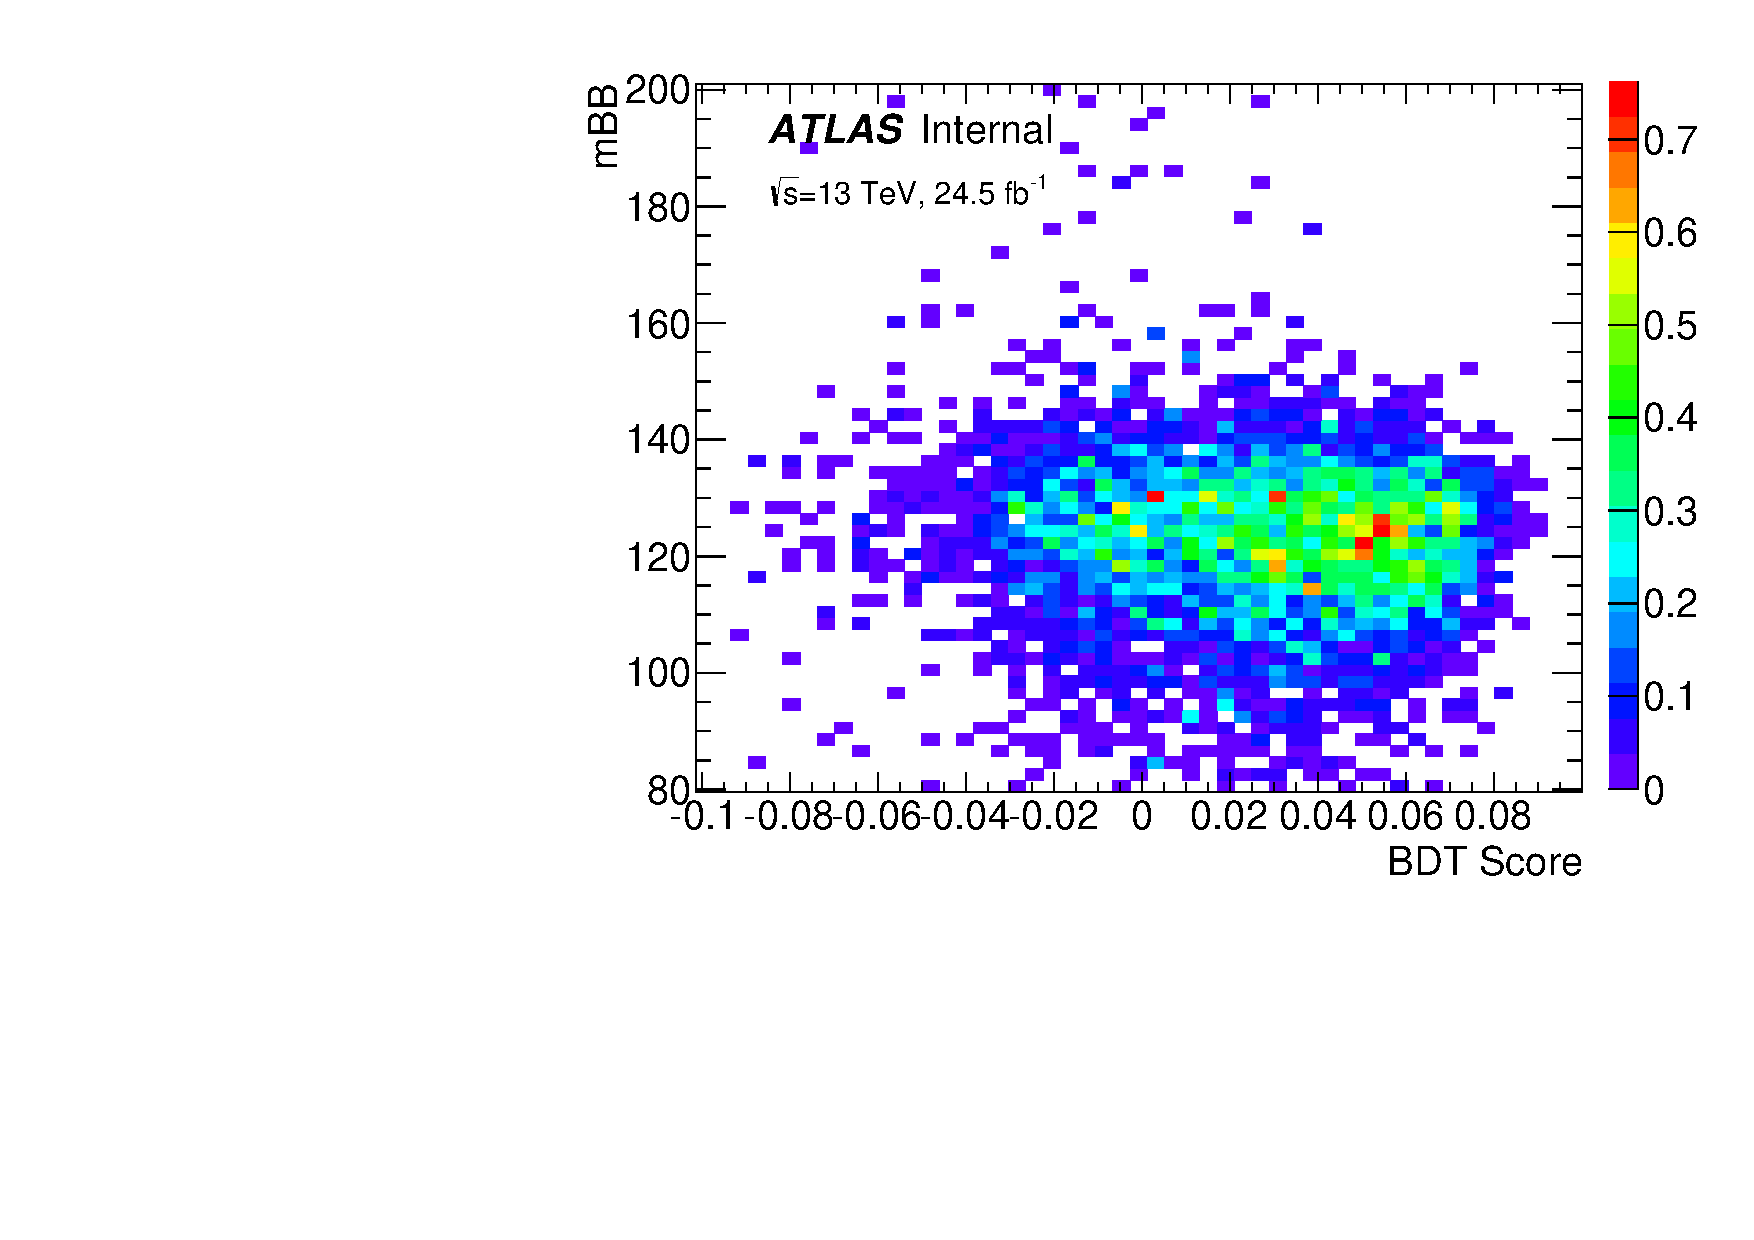
\includegraphics[width=0.48\textwidth]{figures/Mbb_BDT_VBF_2cen.pdf}
 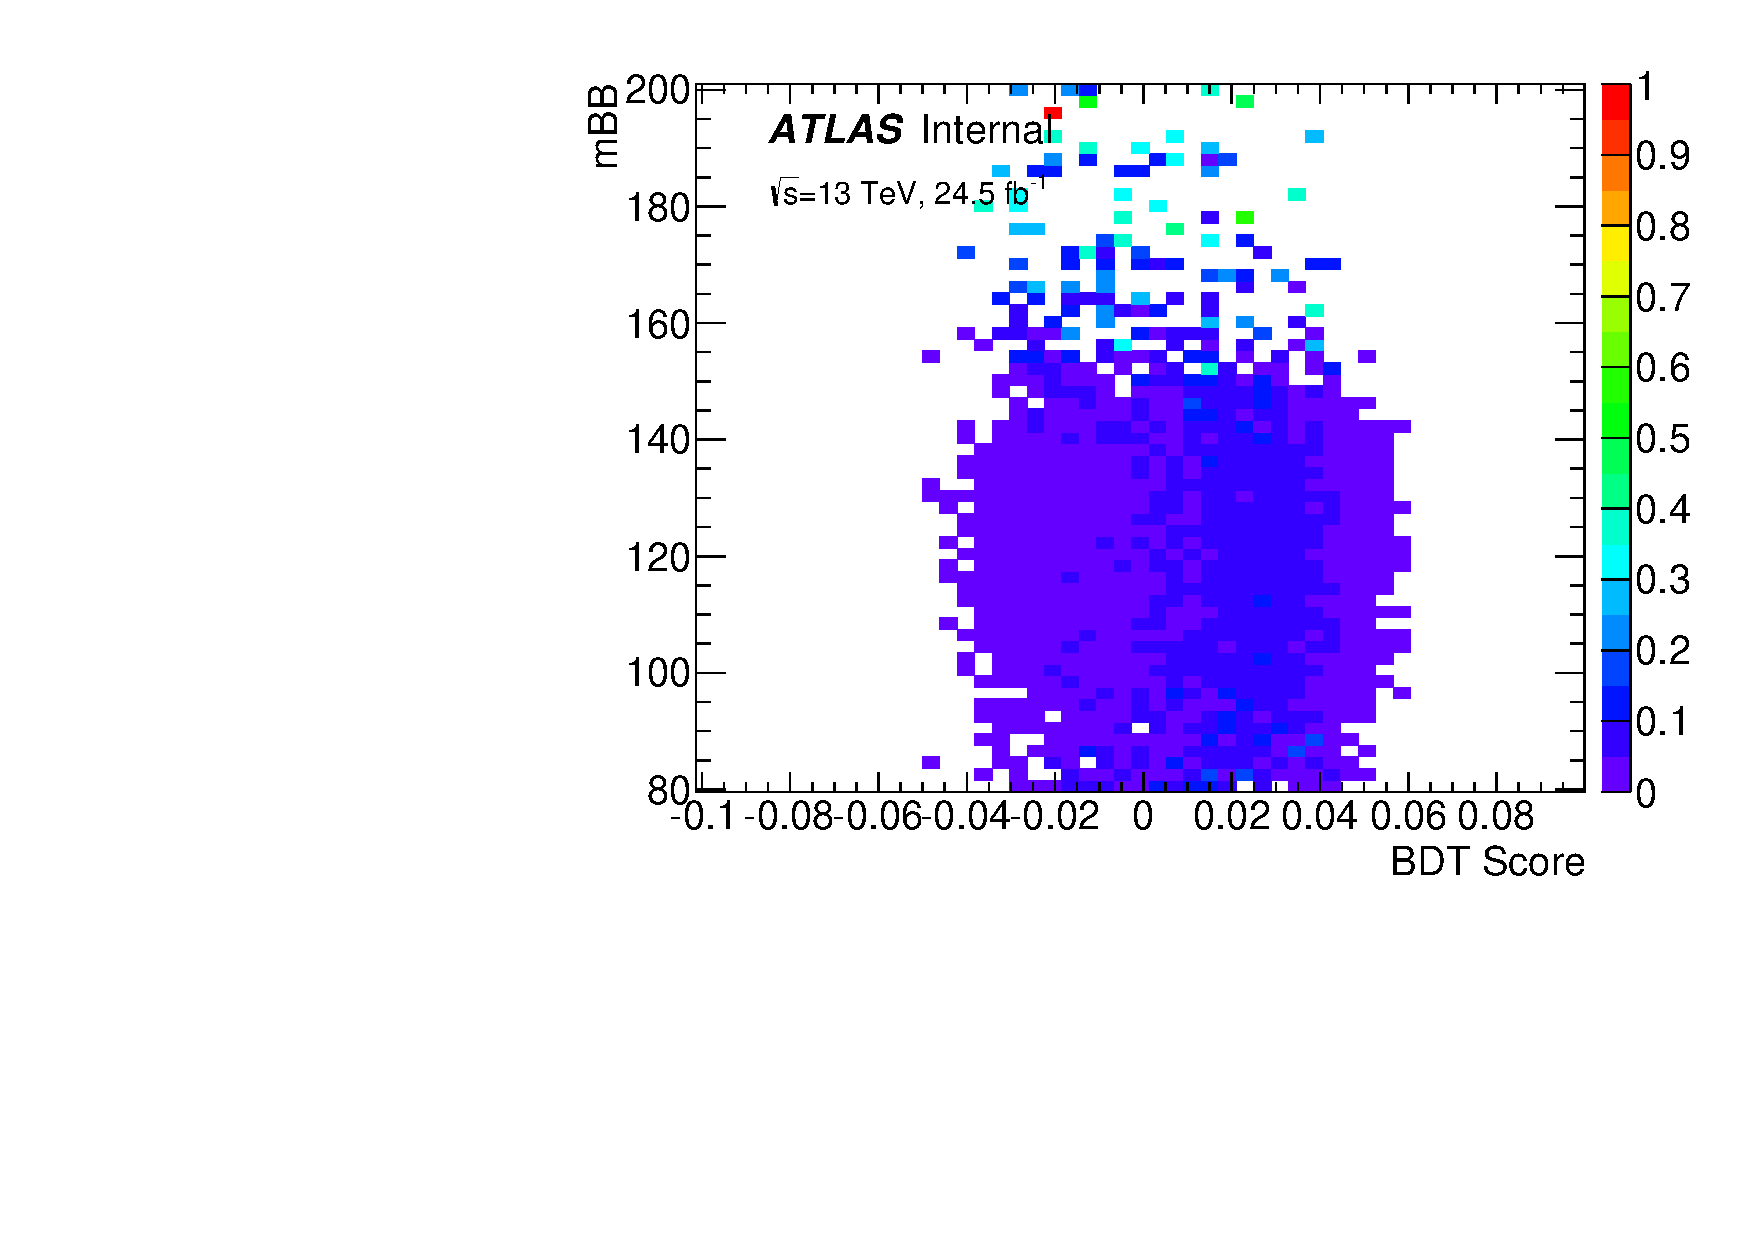
\includegraphics[width=0.48\textwidth]{figures/Mbb_BDT_RowNorm_VBF_2cen.pdf}\\
 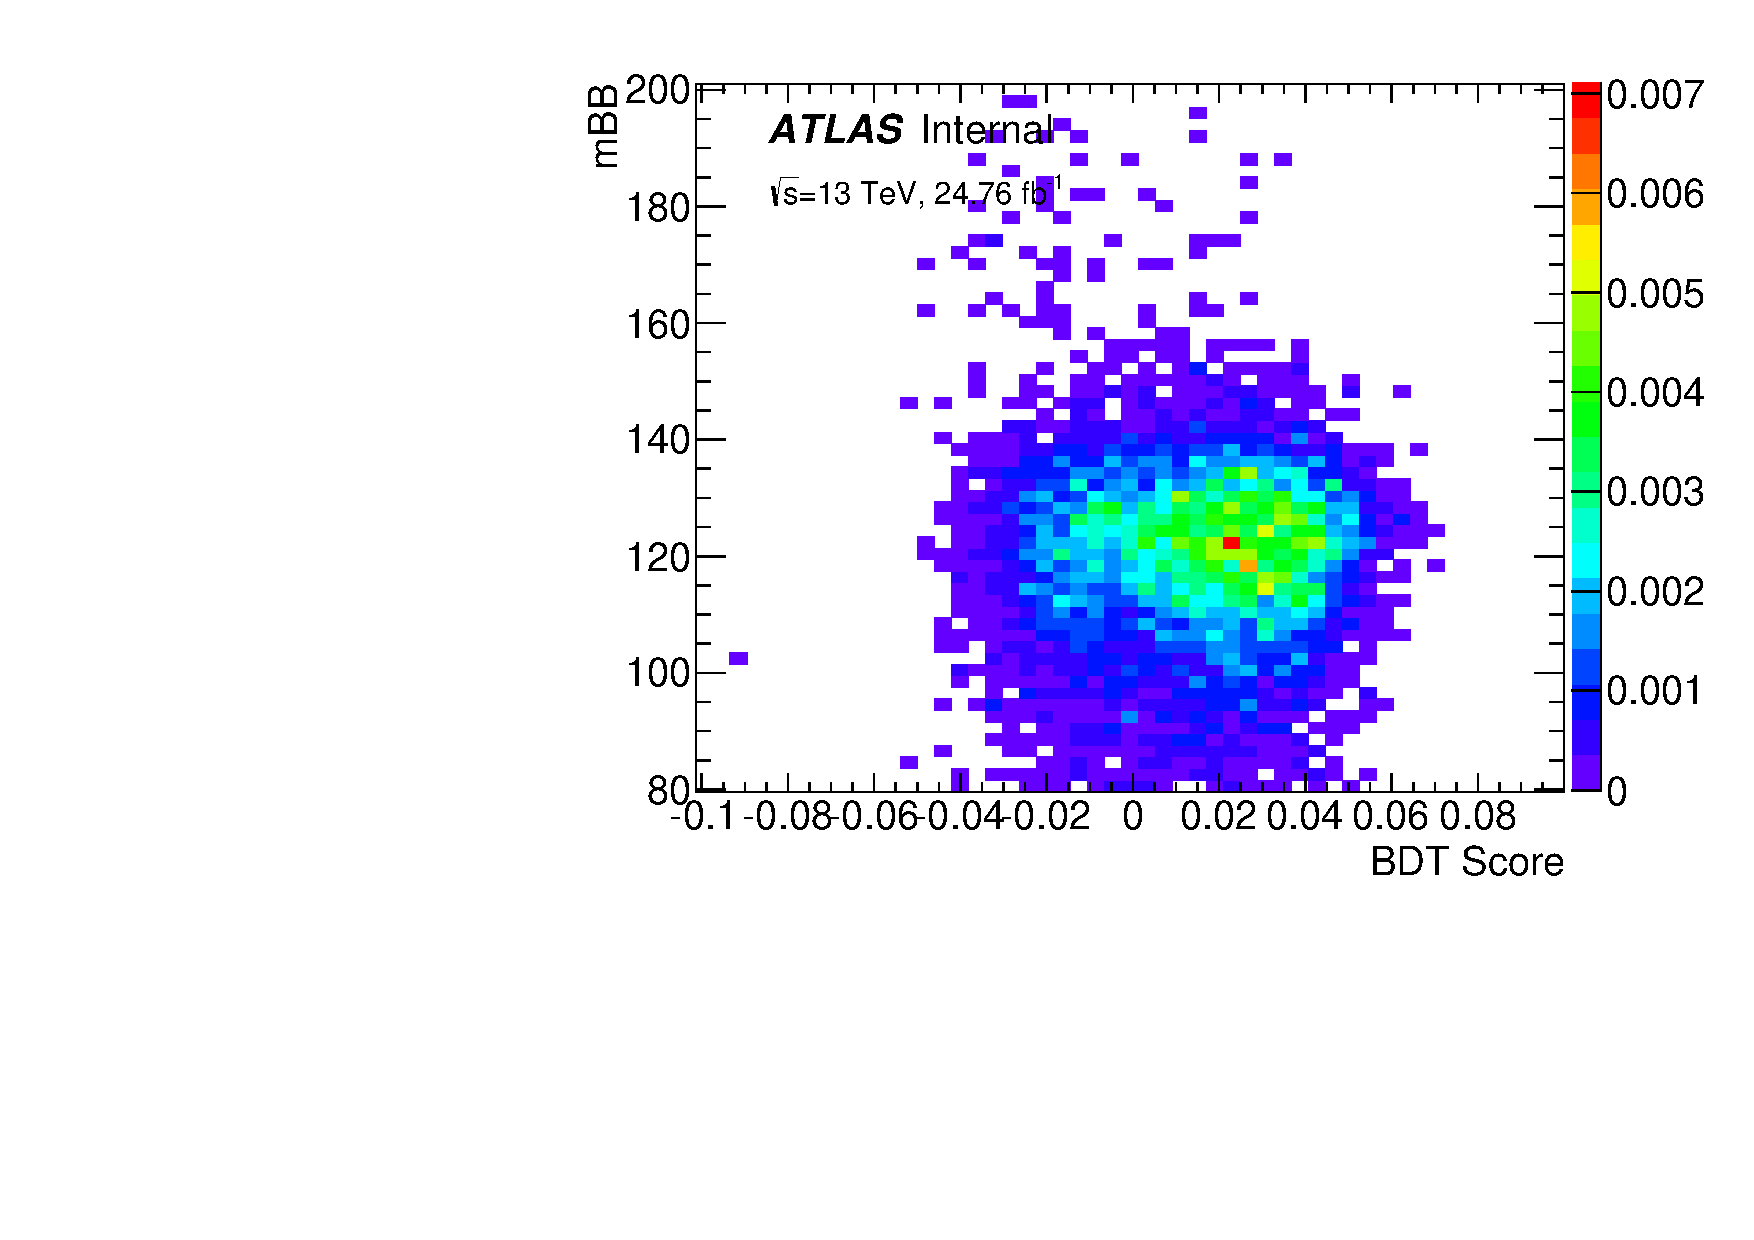
\includegraphics[width=0.48\textwidth]{figures/Mbb_BDT_VBF_4cen.pdf}
 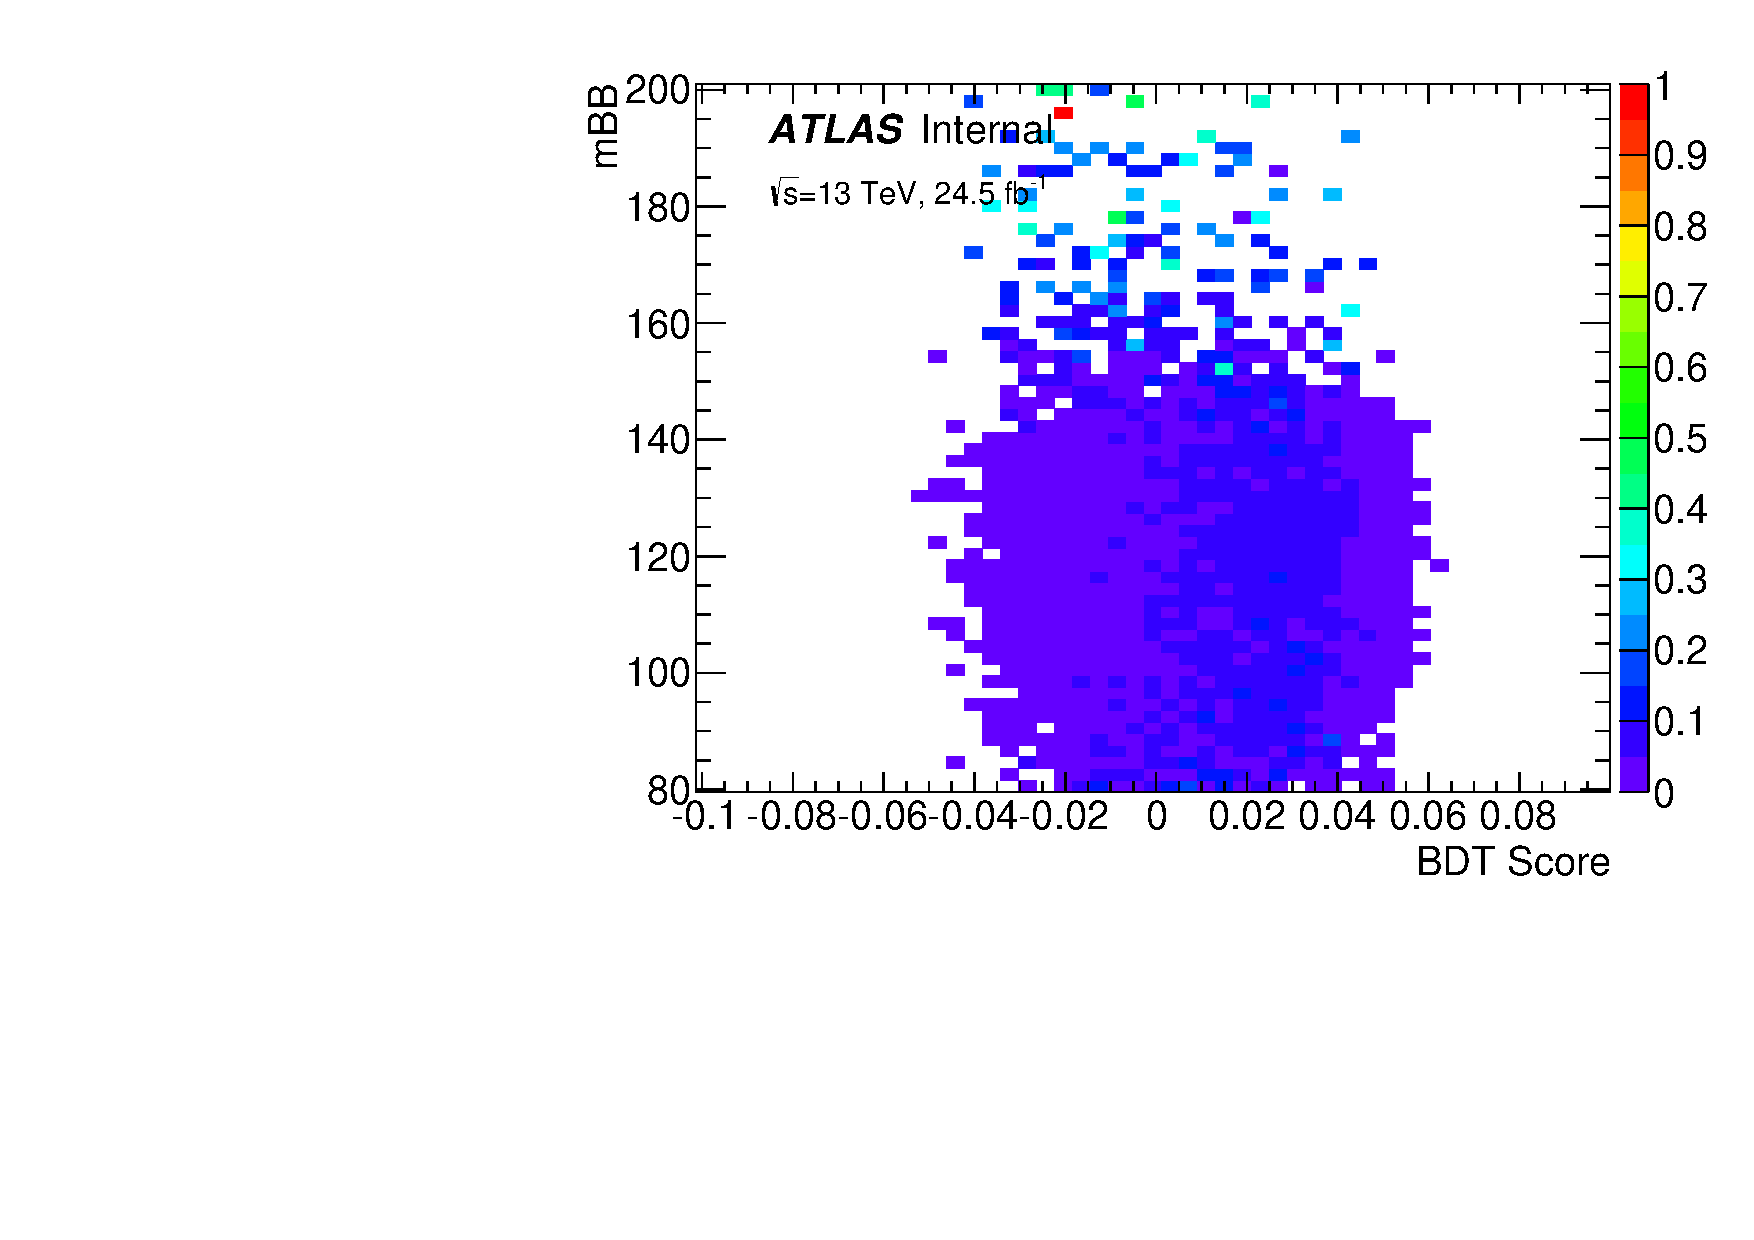
\includegraphics[width=0.48\textwidth]{figures/Mbb_BDT_RowNorm_VBF_4cen.pdf}\\

\caption{VBF signal distributions of $M_{b\bar b}$ Vs. BDT Score for 2 central (top) and 4 central (bottom). The nominal distribution is on left and the distribution with integral of each row normalized to 1 is on right.}
  \label{fig:Mbb_BDT_VBF}
\end{figure}


\begin{figure}[htbp]
  \centering
 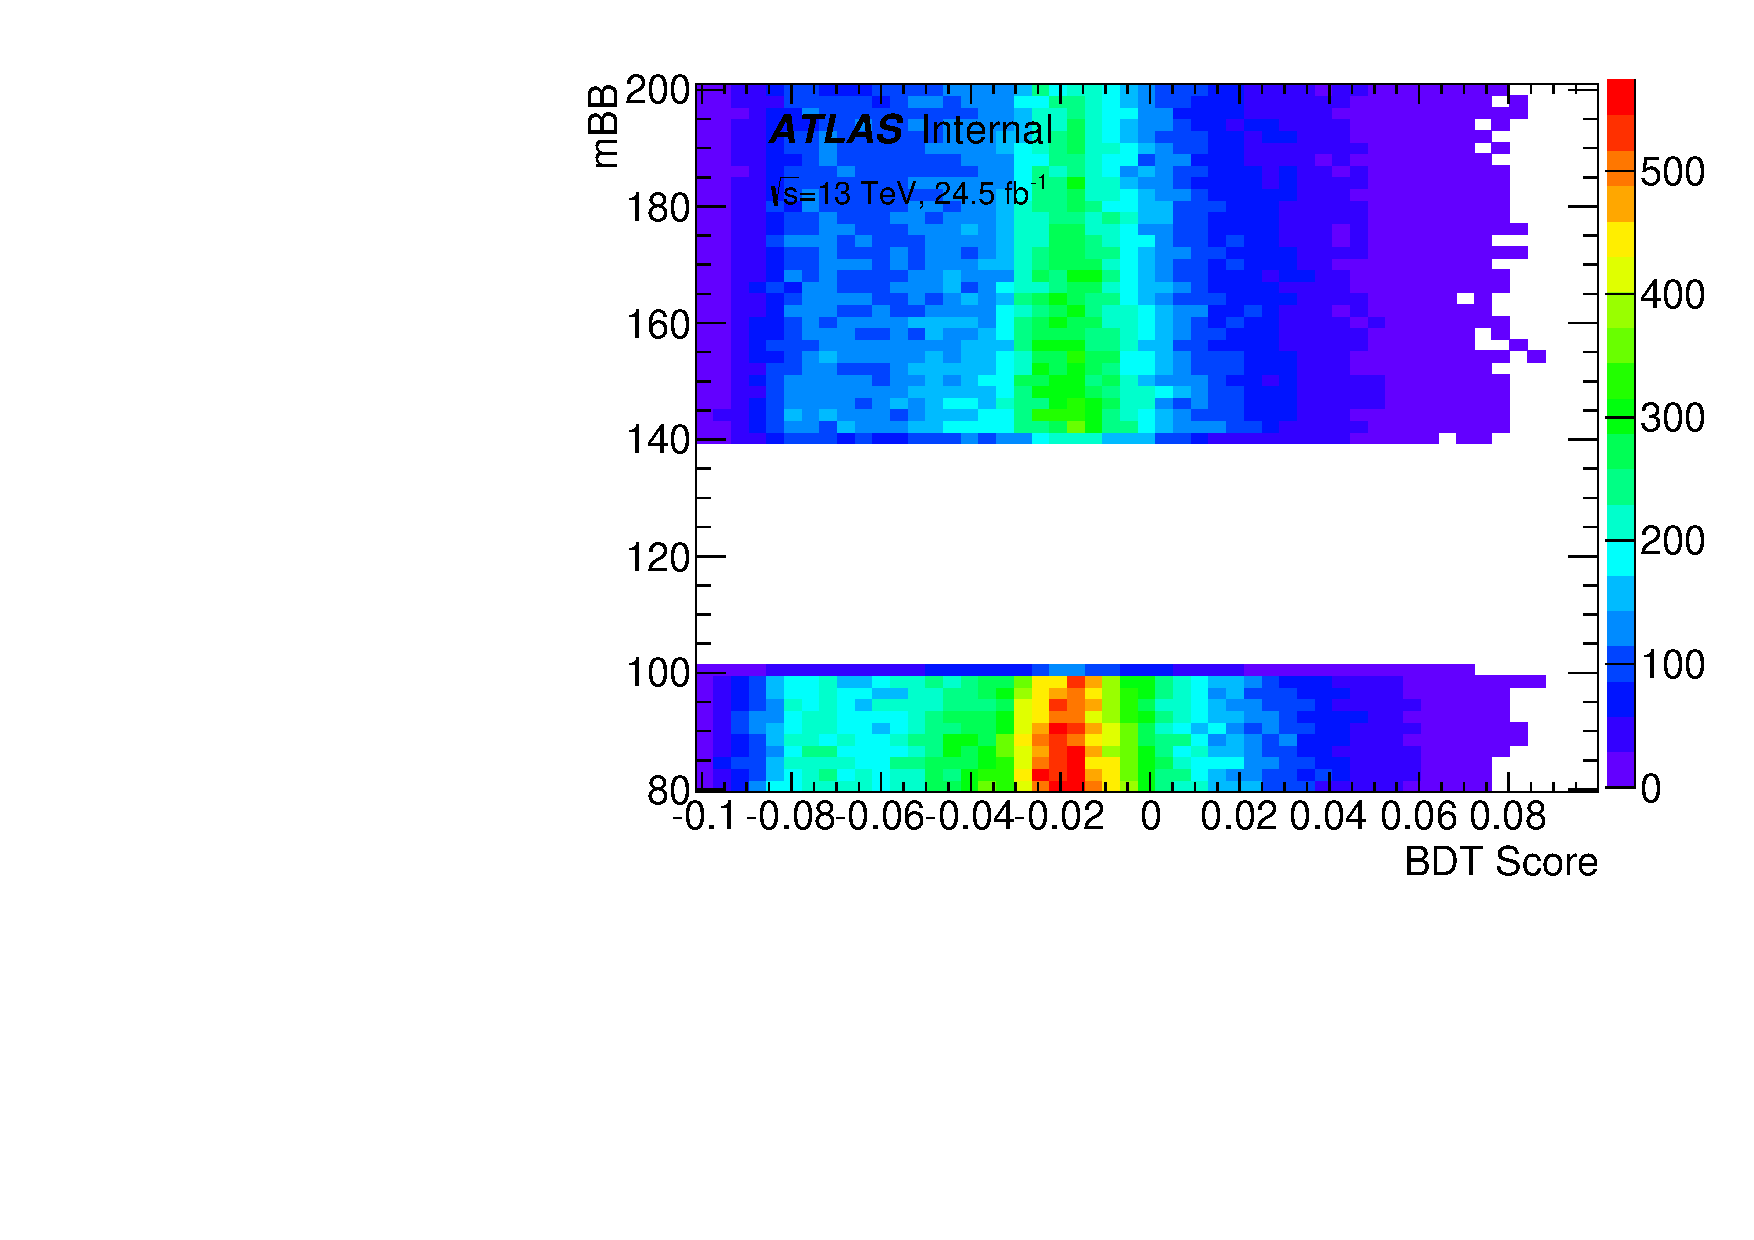
\includegraphics[width=0.48\textwidth]{figures/Mbb_BDT_data_2cen.pdf}
 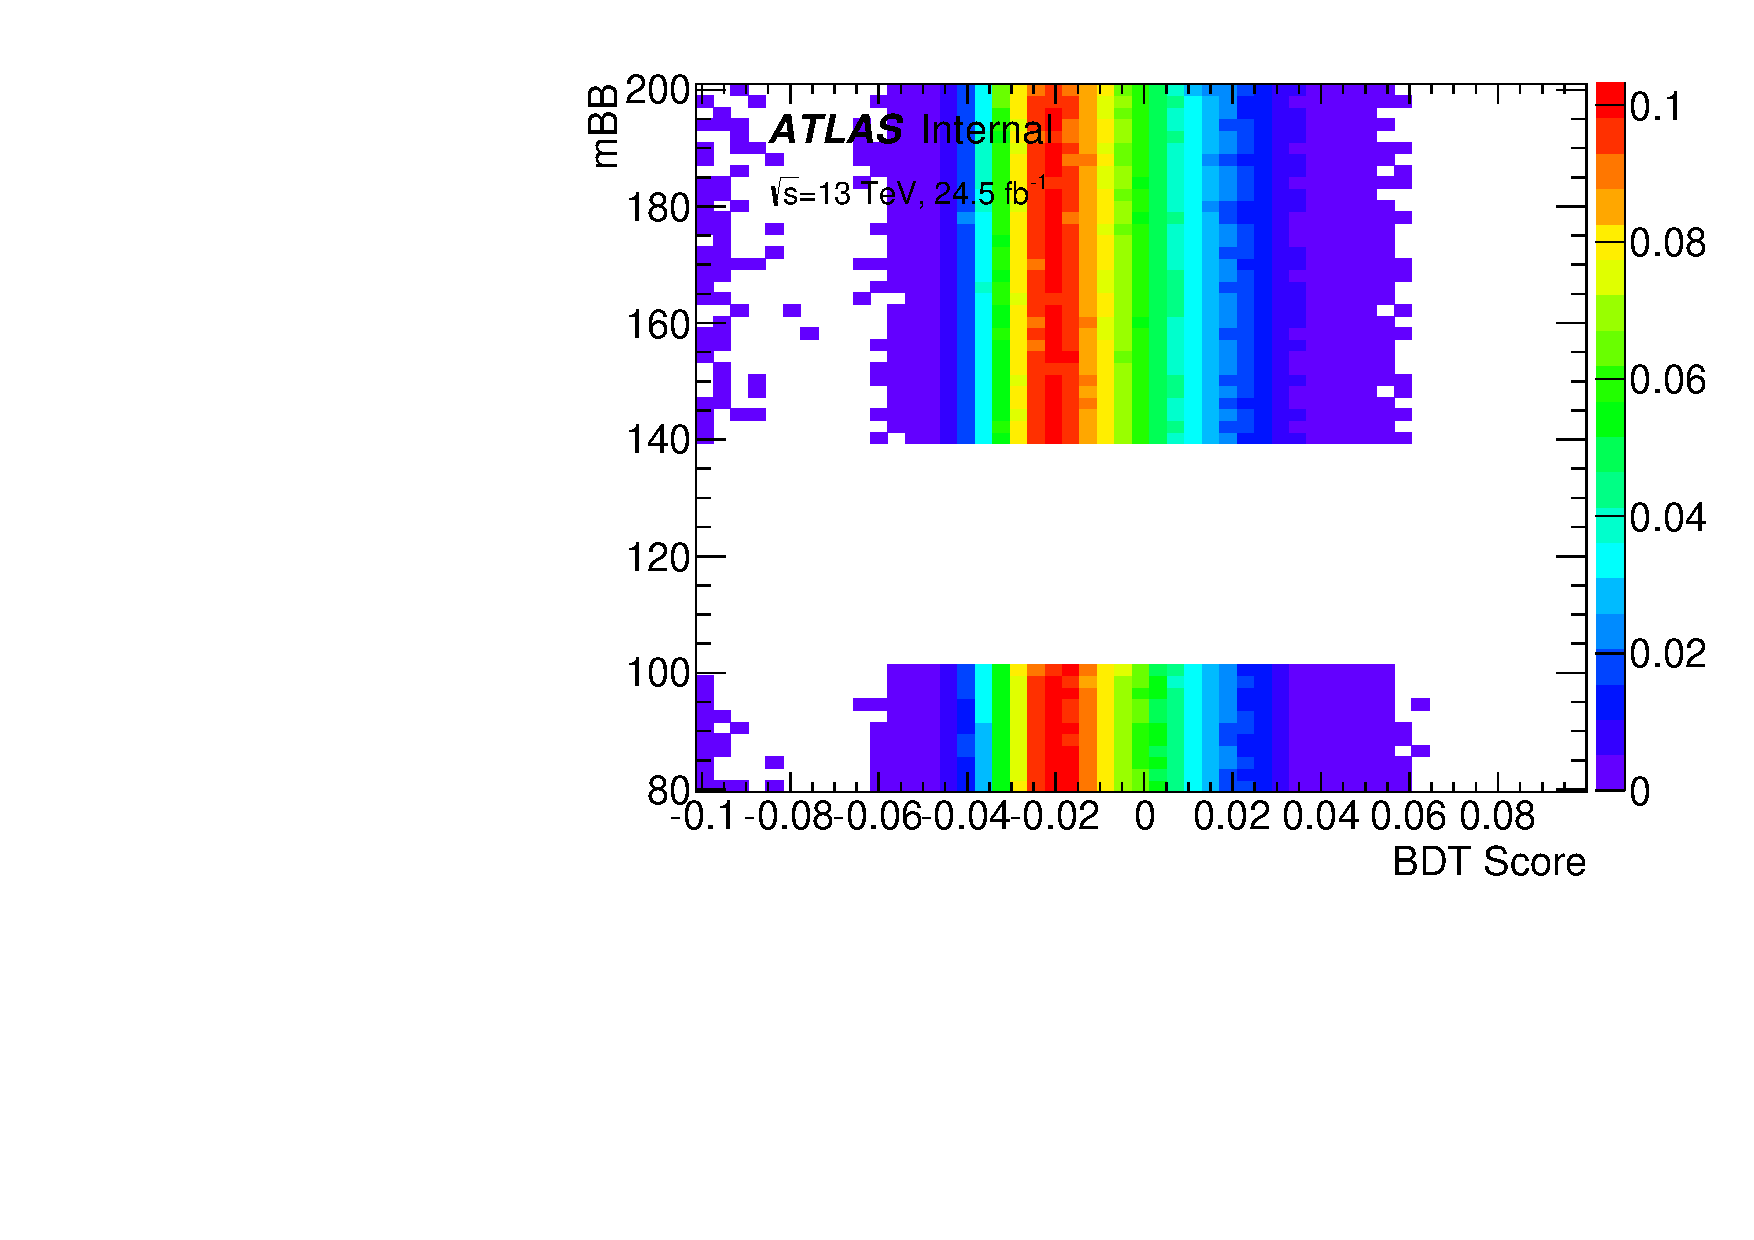
\includegraphics[width=0.48\textwidth]{figures/Mbb_BDT_RowNorm_data_2cen.pdf}\\
 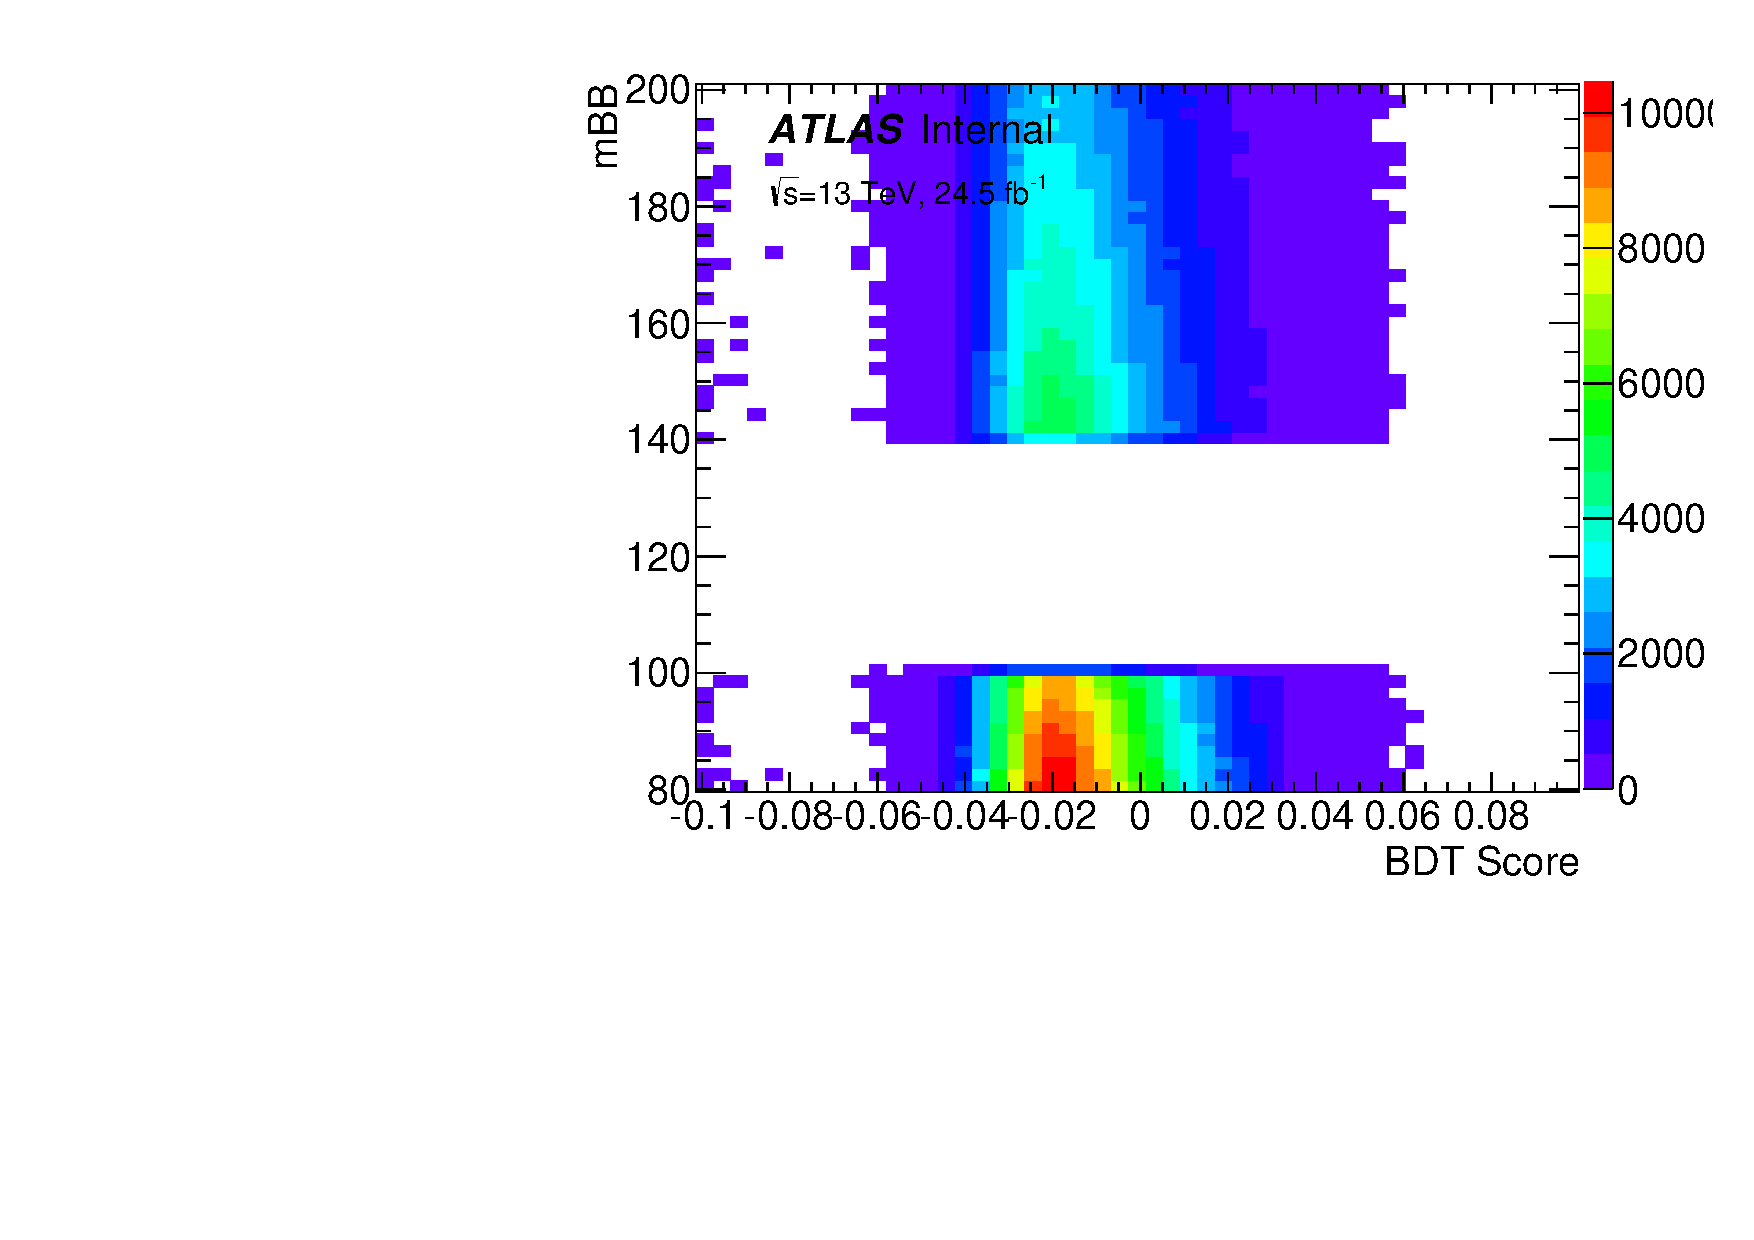
\includegraphics[width=0.48\textwidth]{figures/Mbb_BDT_data_4cen.pdf}
 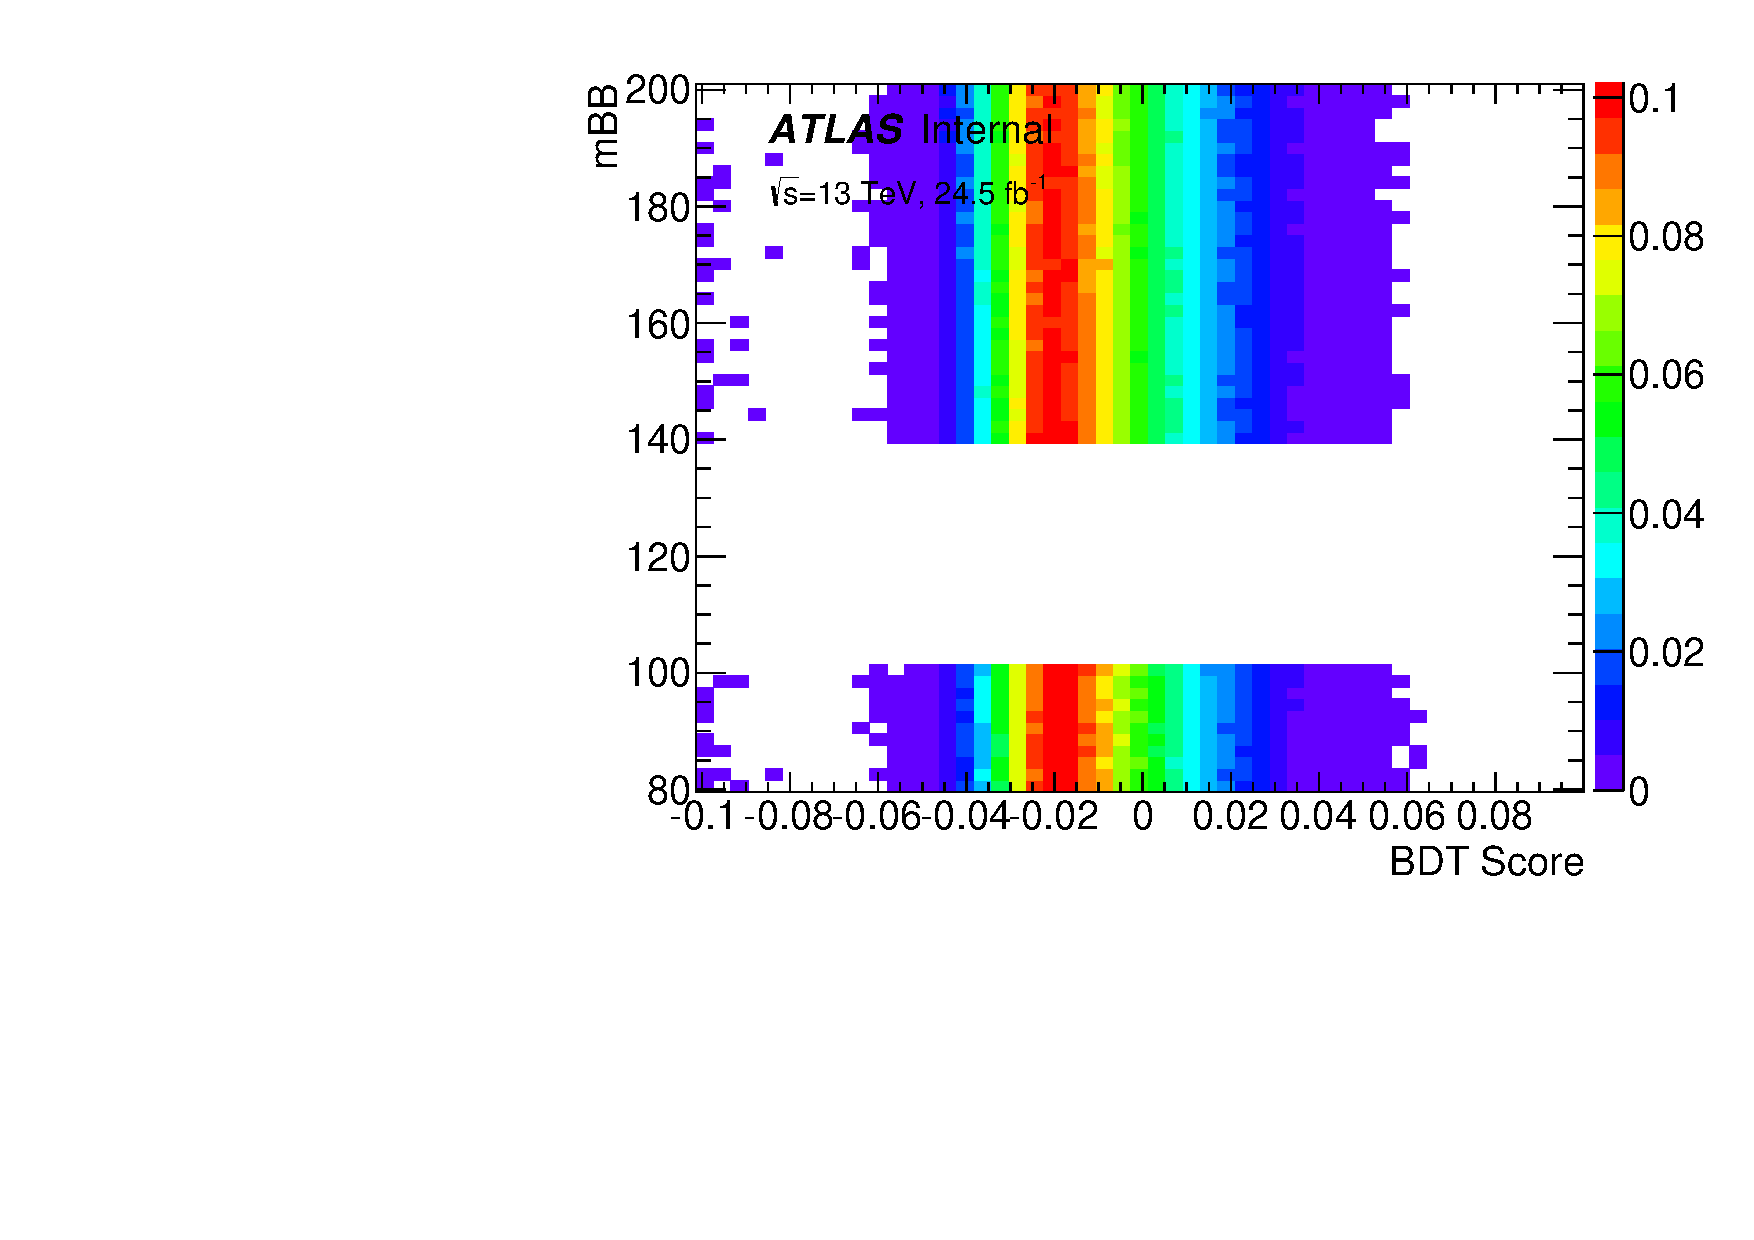
\includegraphics[width=0.48\textwidth]{figures/Mbb_BDT_RowNorm_data_4cen.pdf}\\

\caption{Data distributions of $M_{b\bar b}$ Vs. BDT Score for 2 central (top) and 4 central (bottom). The nominal distribution is on left and the distribution with integral of each row normalized to 1 is on right.}
  \label{fig:Mbb_BDT_data}
\end{figure}


\begin{figure}[htbp]
  \centering
 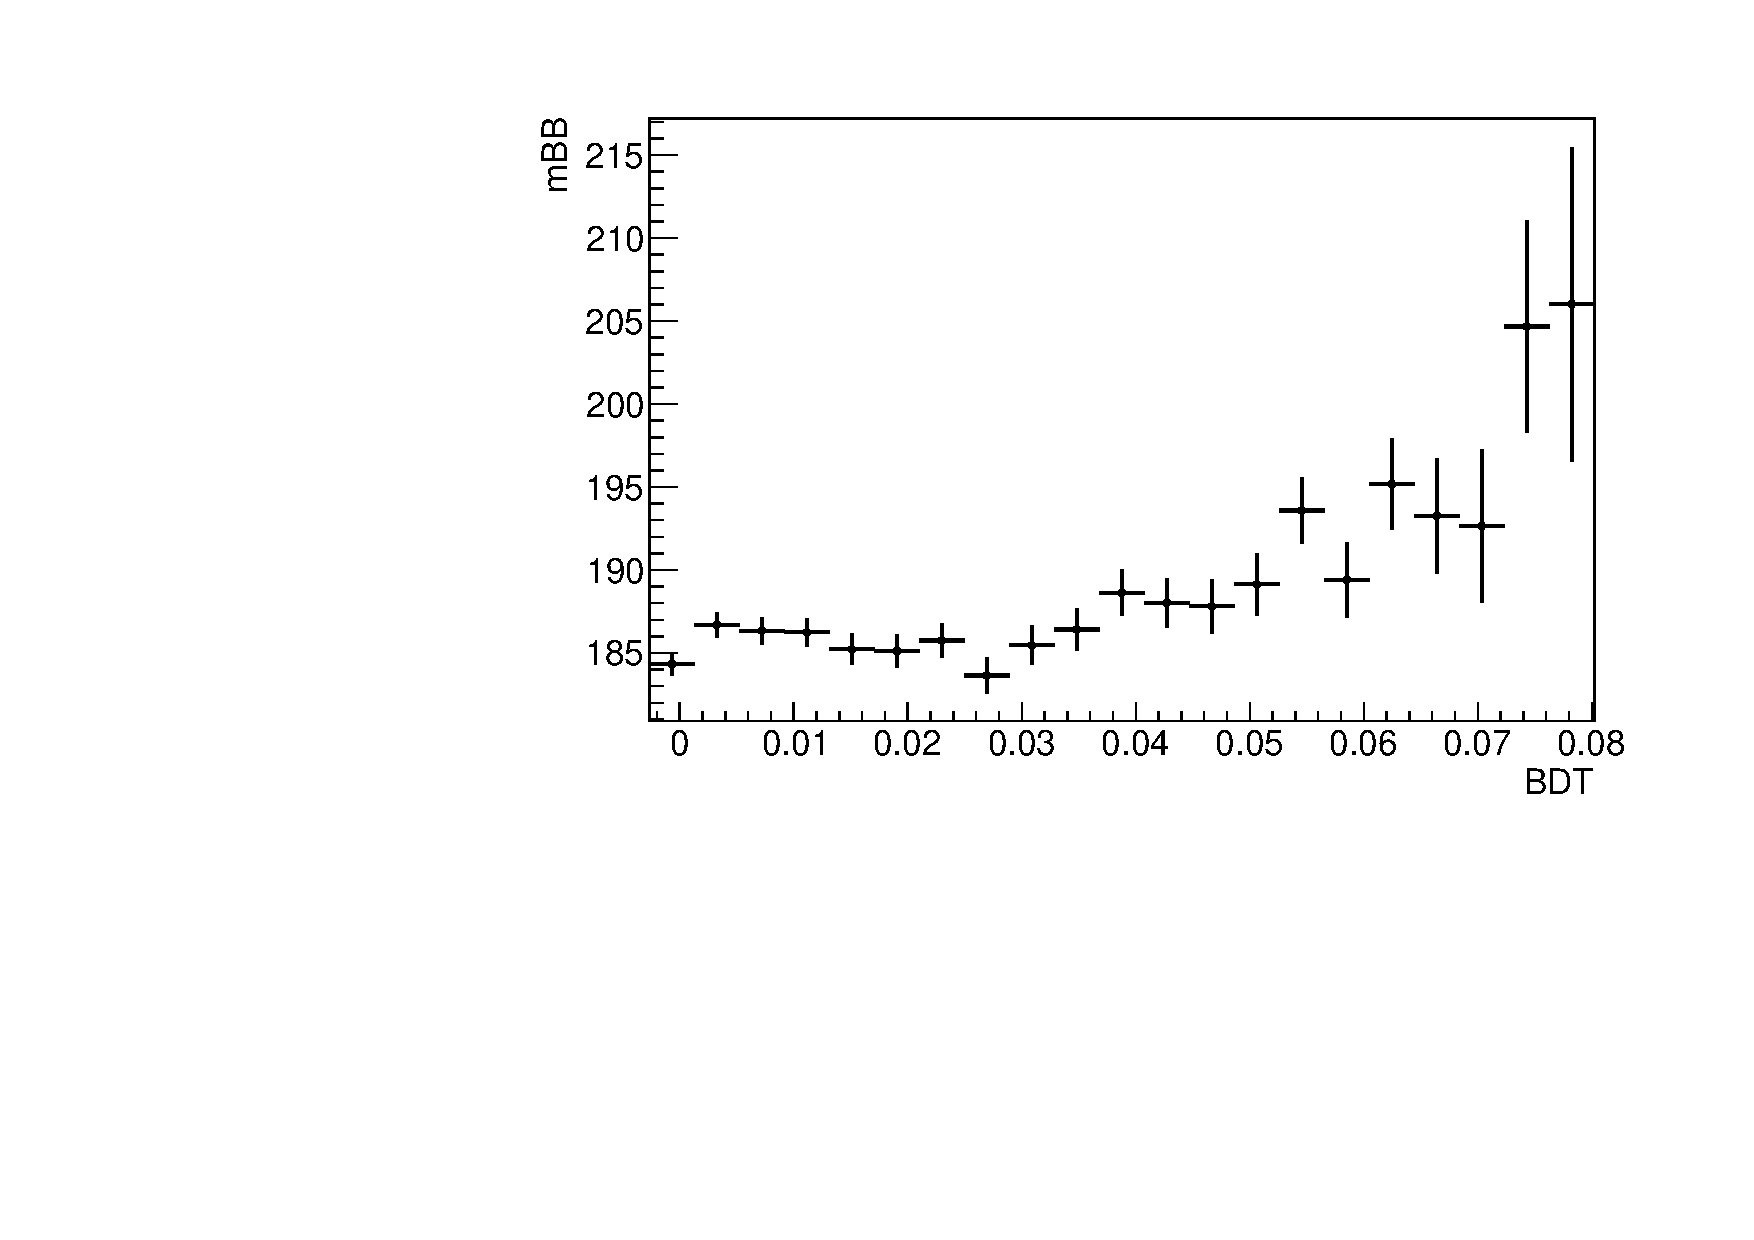
\includegraphics[width=0.48\textwidth]{figures/Profile_BDT_mBB.pdf}
 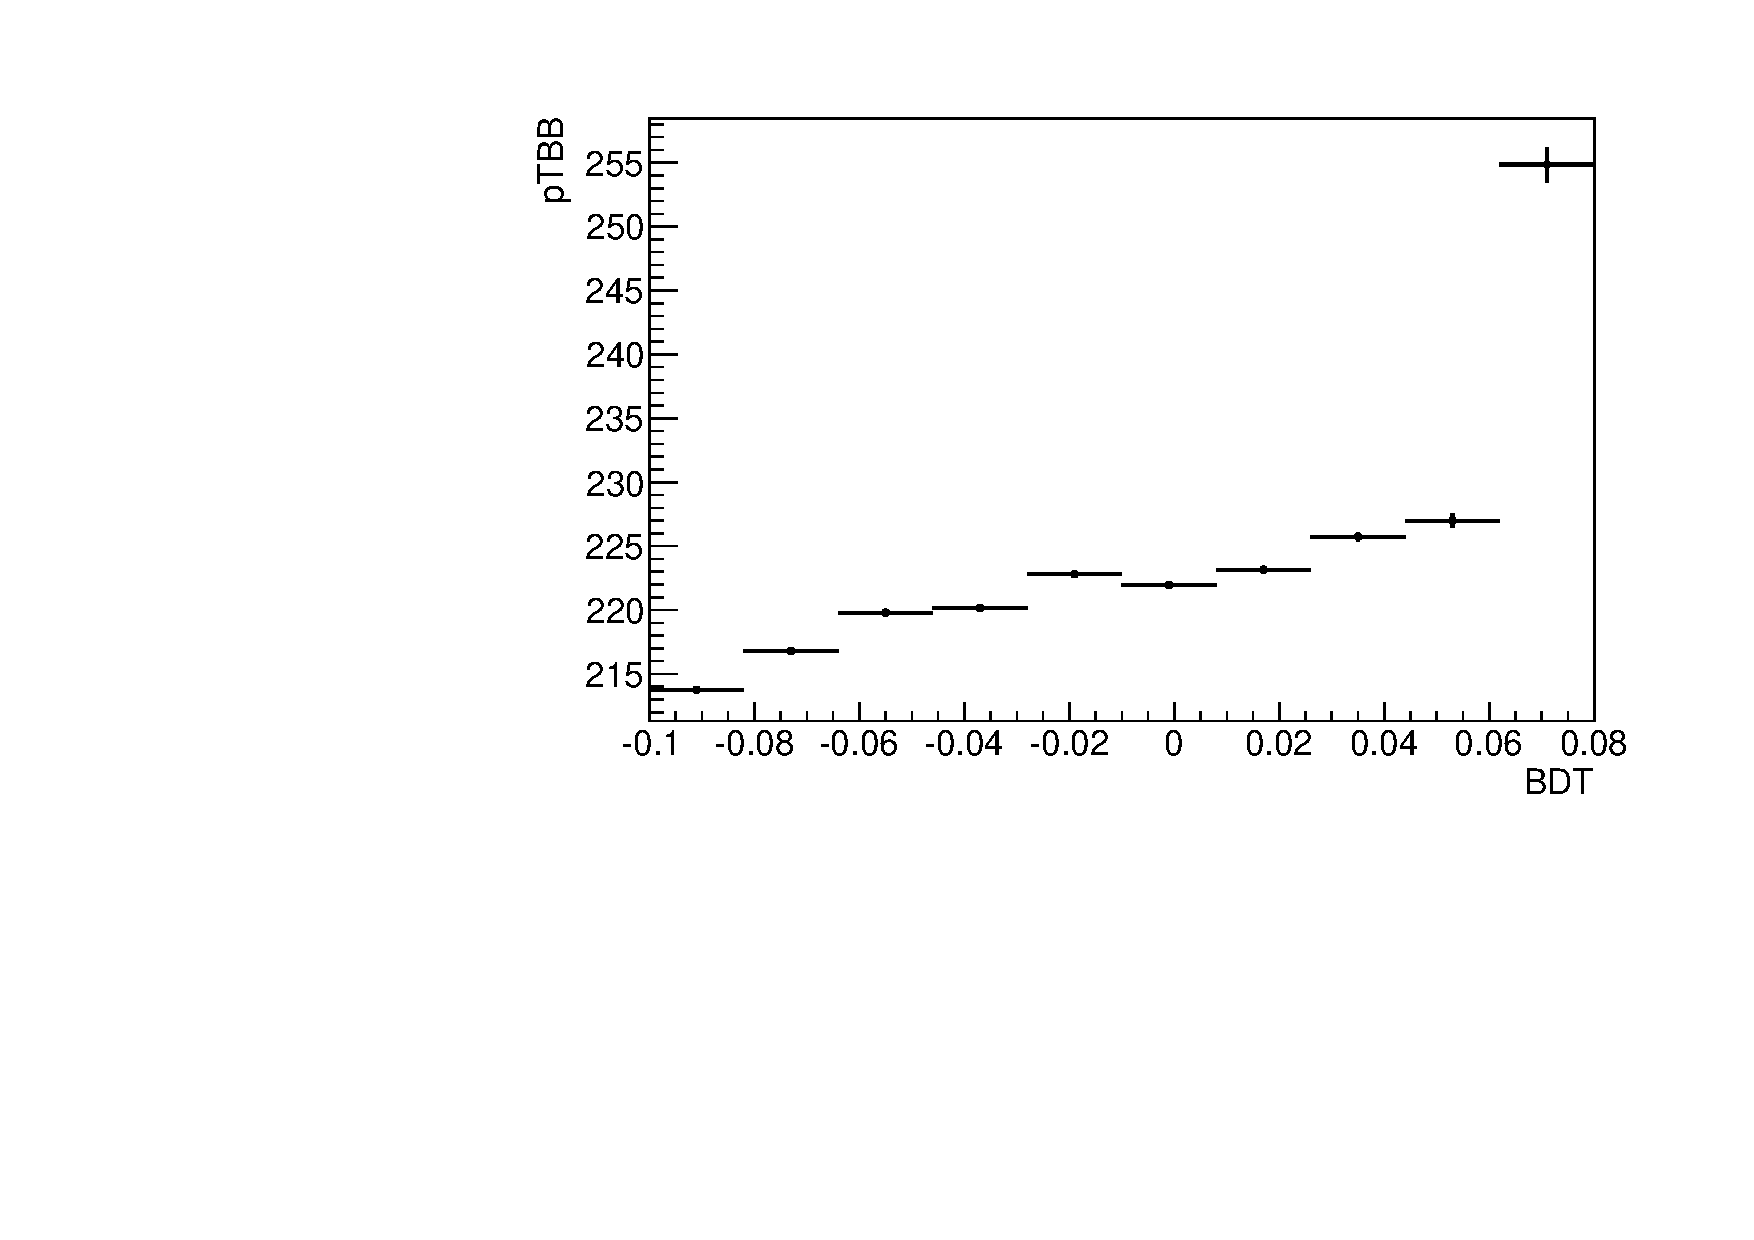
\includegraphics[width=0.48\textwidth]{figures/Profile_BDT_pTBB.pdf}\\

\caption{Profile plots for \Mbb(left) and \pTbb(right) vs. the BDT discriminant for \twocentral channel}
  \label{fig:BDT_Profile}
\end{figure}


\begin{figure}[htbp]
  \centering
 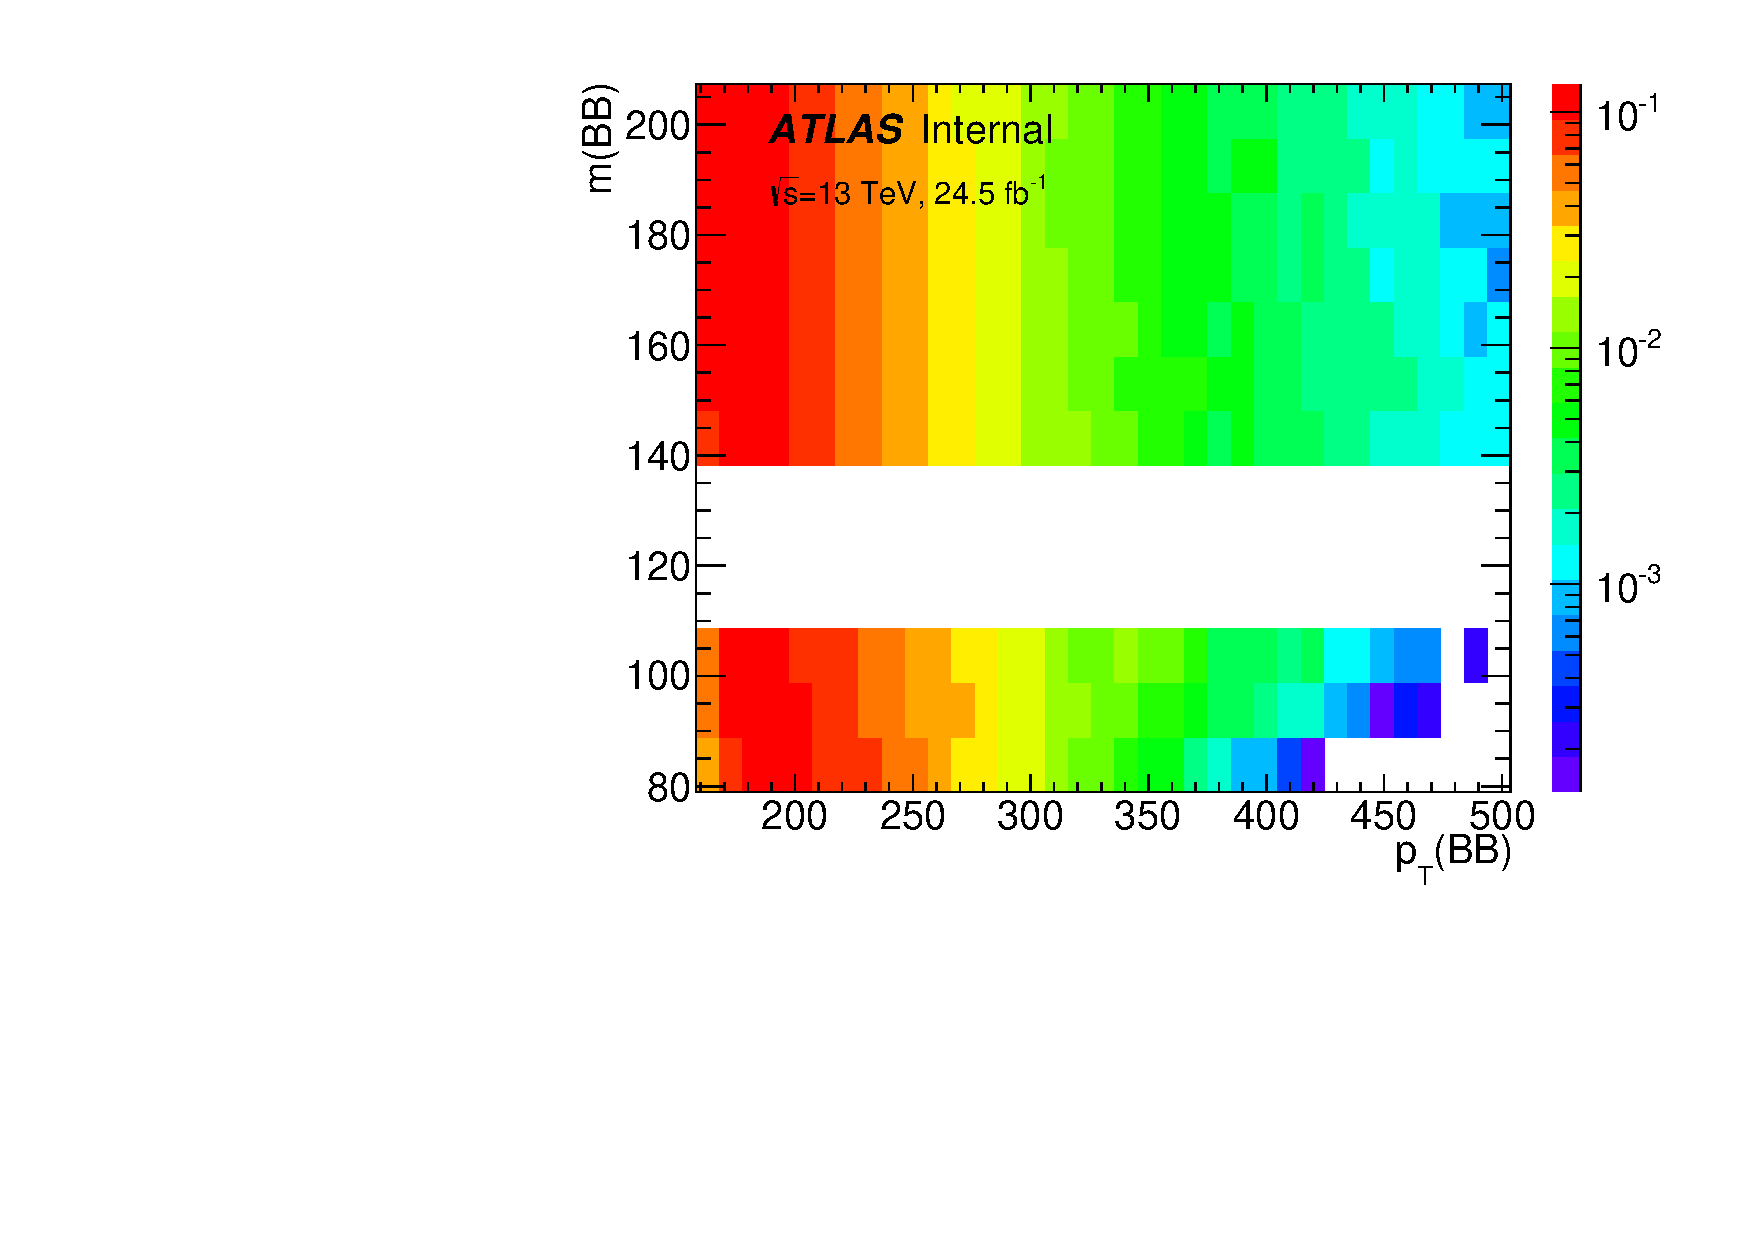
\includegraphics[width=0.6\textwidth]{figures/MBB_pTBB.pdf}
\caption{\twocentral channel \Mbb vs. \pTbb}
  \label{fig:MBB_pTBB}
\end{figure}


\begin{table}[]
\centering
\caption{The sensitivity ($S/\sqrt(B)$) of \twocentral BDT leaving out one input variable at a time. The sensitivity is estimated with cuts retaining top 20\%, 20\%-40\% and top 40\% events of VBF signal events.}
\label{tab:BDT-2cen-sensitivity}
\begin{tabular}{l|l|l|l|}
\cline{2-4}
 & $S/\sqrt(B)$      & Top 20\% & 20\%-40\% \\ \cline{2-4} 
 & $p_T$ balance     & 0.75     & 0.46      \\ \cline{2-4} 
 & $p_{JJ}$          & 0.77     & 0.48      \\ \cline{2-4} 
 & min$\Delta R$(J1) & 0.79     & 0.44      \\ \cline{2-4} 
 & min$\Delta R$(J2) & 0.77     & 0.46      \\ \cline{2-4} 
 & Max($\eta$)       & 0.82     & 0.49      \\ \cline{2-4} 
 & $m_{JJ}$          & 0.77     & 0.47      \\ \cline{2-4} 
 & $\eta^*$          & 0.80     & 0.49      \\ \cline{2-4} 
 & $\Delta m_{JJ}$   & 0.82     & 0.45      \\ \cline{2-4} 
 & $\cos{\theta}$    & 0.79     & 0.50      \\ \cline{2-4} 
 & NTrk500(J2)       & 0.81     & 0.48      \\ \cline{2-4} 
 & Full              & 0.83     & 0.49      \\ \cline{2-4} 
\end{tabular}
\end{table}


\begin{table}[]
\centering
\caption{The sensitivity ($S/\sqrt(B)$) of \fourcentral BDT leaving out one input variable at a time (esimated using Post-ICHEP data). The sensitivity is estimated with cuts retaining top 20\%, 20\%-40\% and top 40\% events of VBF signal events.}
\label{tab:BDT-4cen-sensitivity}
\begin{tabular}{l|l|l|l|}
\cline{2-4}
 & $S/\sqrt(B)$      & Top 20\% & 20\%-40\% \\ \cline{2-4} 
 & $p_T$ balance     & 0.54     & 0.41      \\ \cline{2-4} 
 & $p_{JJ}$          & 0.53     & 0.40      \\ \cline{2-4} 
 & min$\Delta R$(J1) & 0.55     & 0.4       \\ \cline{2-4} 
 & min$\Delta R$(J2) & 0.56     & 0.43      \\ \cline{2-4} 
 & Max($\eta$)       & 0.59     & 0.42      \\ \cline{2-4} 
 & $m_{JJ}$          & 0.58     & 0.41      \\ \cline{2-4} 
 & $\eta^*$          & 0.65     & 0.39      \\ \cline{2-4} 
 & $\Delta m_{JJ}$   & 0.55     & 0.3       \\ \cline{2-4} 
 & $\cos{\theta}$    & 0.62     & 0.42      \\ \cline{2-4} 
 & NTrk500(J1)       & 0.65     & 0.40      \\ \cline{2-4} 
 & NTrk500(J2)       & 0.53     & 0.42      \\ \cline{2-4} 
 & HT                & 0.57     & 0.31      \\ \cline{2-4} 
 & Full              & 0.69     & 0.39      \\ \cline{2-4} 
\end{tabular}
\end{table}


\begin{table}[]
\centering
\caption{The sensitivity ($S/\sqrt(B)$) of \twocentral BDT 3-fold test}
\label{tab:BDT-2cen-kfold}
\begin{tabular}{l|l|l|l|l|}
\cline{2-5}
 & $S/\sqrt(B)$ & Test 1 & Test 2 & Test 3 \\ \cline{2-5} 
 & Top 30\%     & 0.80   & 0.80   & 0.82   \\ \cline{2-5} 
 & 30\%-40\%    & 0.31   & 0.31   & 0.30   \\ \cline{2-5} 
\end{tabular}
\end{table}


\begin{table}[]
\centering
\caption{The sensitivity ($S/\sqrt(B)$) of \fourcentral BDT 3-fold test}
\label{tab:BDT-4cen-kfold}
\begin{tabular}{l|l|l|l|l|}
\cline{2-5}
 & $S/\sqrt(B)$ & Test 1 & Test 2 & Test 3 \\ \cline{2-5} 
 & Top 20\%     & 0.55   & 0.54   & 0.54   \\ \cline{2-5} 
 & 20\%-40\%    & 0.39   & 0.39   & 0.37   \\ \cline{2-5} 
\end{tabular}
\end{table}


\begin{figure}[htbp]
  \centering
 \includegraphics[width=0.45\textwidth]{figures_final/Canv_Giacinto_Check_ratio_2cen.png}
 \includegraphics[width=0.45\textwidth]{figures_final/Canv_Giacinto_Check_ratio_4cen.png}
\caption{Number of events in sidebands of training and test sample. The numbers of events predicted by BDT in training and test data samples are mostly statistically compatible. The most prominent difference is in SRI of \fourcentral region and is only $2\%$.}
  \label{fig:bdt_evt_sidebands}
\end{figure}

\begin{figure}[htbp]
  \centering
 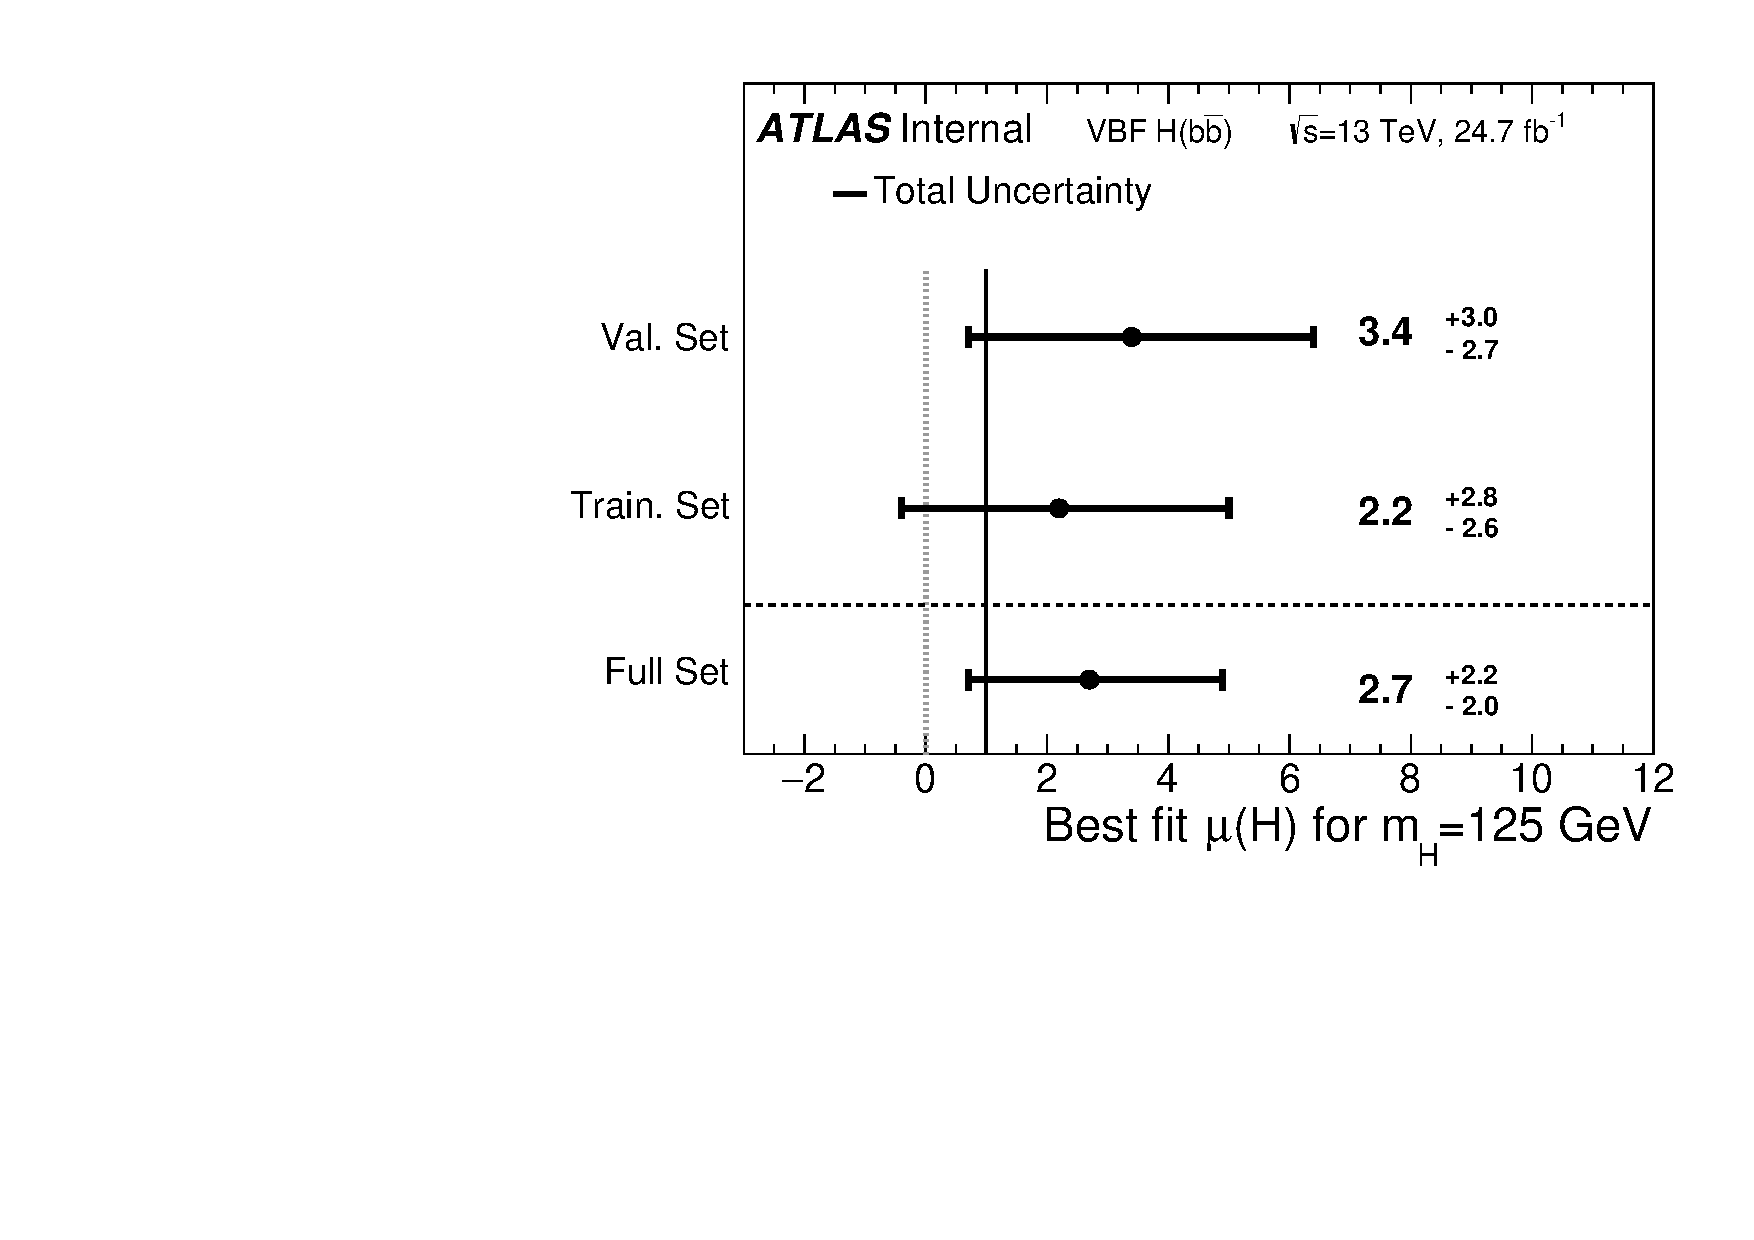
\includegraphics[width=0.6\textwidth]{figures_final/Plot_mu_summary_Giacinto.pdf}
\caption{Data training and test sample fit summary. The fitted Higgs strengths obtained from full, training and test datasets are compatible within the uncertainties.}
  \label{fig:separatefit}
\end{figure}
